\clearpage
\section{Techniki tworzenia skalowalnych aplikacji webowych}

Przed przystąpieniem do implementacji projektu inżynierskiego, istotne jest zrozumienie technik i narzędzi stosowanych w tworzeniu nowoczesnych, skalowalnych aplikacji webowych. Opisane poniżej elementy znalazły zastosowanie w ramach niniejszej pracy.

\subsection{Architektura mikroserwisowa}

Przez lata pojawiło się wiele definicji architektury oprogramowania. Panowie Bass, Clements i Kazman w 2003 roku \cite{bass2012software} wyjaśnili to pojęcie, podkreślając, że

\begin{displayquote}
\emph{Architektura oprogramowania programu lub systemu informatycznego jest strukturą lub zbiorem struktur tego systemu, obejmującym elementy oprogramowania, widoczne dla pozostałych elementów oprogramowania oraz zależności między nimi.}
\end{displayquote}

Architektura mikroserwisowa to podejście do strukturyzacji aplikacji jako zbiór niewielkich, niezależnych usług, które komunikują się ze sobą przy użyciu standardowych protokołów komunikacji synchronicznej, takich jak HTTP/gRPC \cite{grpc} lub asynchronicznych kolejek komunikatów, np. RabbitMQ \cite{rabbitmq}/Apache Kafka \cite{kafka}. Każdy mikroserwis jest odpowiedzialny za wykonanie określonej funkcjonalności lub usługi i może być rozwijany, wdrażany oraz zarządzany niezależnie od innych. Ta architektura zapewnia wysoką skalowalność i elastyczność, umożliwiając łatwe wprowadzanie zmian i adaptację do zmieniających się wymagań. Mikroserwisy przechowujące dane często mają swoje własne bazy danych, co zwiększa ich niezależność i izolację od innych części systemu.

\begin{figure}[!h]
    \centering 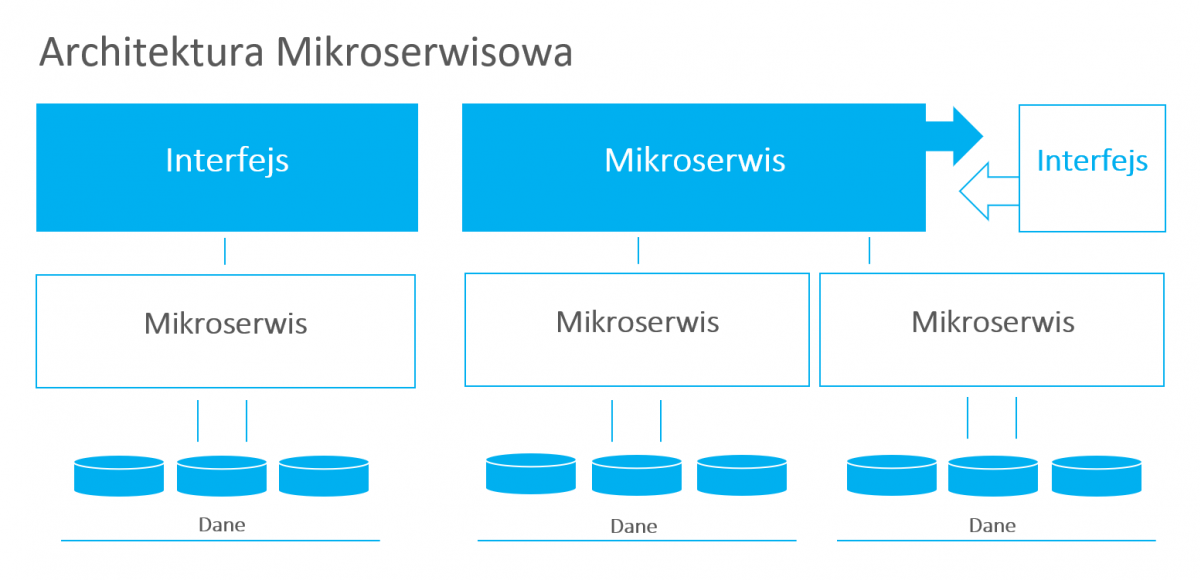
\includegraphics[width=1.0\linewidth]{mikroserwisy.png}
    \caption{Reprezentacja graficzna systemu o architekturze mikroserwisowej \cite{microservices_rys}}
\end{figure}


Główną konsekwencją zastosowania takiej architektury, jest możliwości niezależnego poziomego skalowania każdego komponentu systemu, ponieważ każdy serwis jest osobną jednostką wdrożeniową (np. kontenerem).

Z powodu konieczności komunikacji między elementami systemu, często utrudnione jest zastosowanie spójności natychmiastowej, znanej np. z relacyjnych baz danych. W systemach takich stosowana jest tzw. spójność ostateczna (ang. "eventual consistency") \cite{eventual_consistency}. Powoduje ona, że najnowszy odczyt nie gwarantuje otrzymania danych wynikających z najnowszego zapisu. Utrudnia to m.in. tworzenie interfejsów graficznych dla użytkowników końcowych oraz testowanie aplikacji.

Architektura mikroserwisowa sprzyja tworzeniu systemów o wysokiej niezawodności i dostępności. Uruchamiając wielokrotne instancje poszczególnych serwisów, system staje się odporny na chwilowe awarie. Umożliwia to rozłożenie ruchu pomiędzy instancje.

\begin{longtable}{| m{0.15\linewidth} | m{0.4\linewidth} | m{0.4\linewidth} |}
    \caption{Porównanie architektur: mikroserwisowej i monolitycznej.}
    \label{table:architektura_porownanie} \\

    \hline
    Aspekt & Architektura mikroserwisowa & Architektura monolityczna \\ \hline\hline \endfirsthead \endfoot
    \hline \endlastfoot

    Struktura & Podzielona na mniejsze, niezależne usługi. & Jednolita aplikacja, gdzie wszystkie funkcje są ściśle powiązane i działają jako jedna jednostka. \\ \hline
    Skalowalność & Wysoka; poszczególne mikroserwisy mogą być skalowane niezależnie. & Ograniczona; skalowanie często oznacza konieczność skalowania całej aplikacji. \\ \hline
    Zarządzanie & Możliwość niezależnego zarządzania, rozwijania i wdrażania poszczególnych mikroserwisów. & Zarządzanie całością aplikacji odbywa się centralnie. \\ \hline
    Bazy danych & Każdy mikroserwis może mieć własną bazę danych, zwiększając izolację i niezależność. & Zazwyczaj jedna baza danych dla całej aplikacji. \\ \hline
    Złożoność & Większa złożoność w zarządzaniu i koordynacji między serwisami. & Mniejsza złożoność, ponieważ wszystkie komponenty są w jednym miejscu. \\ \hline
    Odporność na awarie & Wysoka; awaria jednego mikroserwisu zazwyczaj nie wpływa na cały system. & Niższa; awaria w jednym miejscu może wpłynąć na całą aplikację. \\ \hline
    Aktualizacje & Możliwość aktualizowania poszczególnych mikroserwisów niezależnie, bez wpływu na resztę systemu. & Aktualizacje wymagają zwykle zatrzymania i aktualizacji całej aplikacji. \\ \hline
    Komunikacja & Używa lekkich protokołów komunikacyjnych, takich jak HTTP/gRPC, kolejki komunikatów. & Komunikacja wewnętrzna jest mniej skomplikowana, ponieważ wszystko jest częścią jednego systemu. \\ \hline
    Rozwój i utrzymanie	& Może być bardziej skomplikowany ze względu na większą liczbę komponentów i ich niezależność. & Prostsze do zarządzania, dopóki aplikacja nie staje się zbyt duża. \\ \hline
    Spójność danych & Często stosuje model „eventual consistency”, co może komplikować pewne aspekty działania aplikacji. & Łatwiejsza do osiągnięcia spójność danych dzięki centralnej bazie danych. \\ \hline
    Niezawodność  & Każdy serwis może być uruchamiany w wielu instancjach, co zwiększa niezawodność i dostępność.		 & Zależy od pojedynczej instancji aplikacji, co może ograniczać niezawodność.
    \\ \hline
\end{longtable}

Architektura mikroserwisowa jest preferowana do tworzenia skalowalnych aplikacji webowych ze względu na jej zdolność do niezależnego skalowania poszczególnych usług i większą odporność na awarie, co zapewnia elastyczność, niezawodność i szybkość adaptacji do zmieniających się potrzeb.

\subsection{Skalowalność}

Skalowanie usług jest ważnym aspektem w projektowaniu i utrzymaniu aplikacji internetowych, zwłaszcza w kontekście rosnącego zapotrzebowania na usługi danej aplikacji, spowodowanego np. wzrostem liczby użytkowników. W kontekście systemów informatycznych skalowanie może być realizowane zarówno w sposób poziomy, jak i pionowy.

Skalowanie Poziome: Oznacza dodawanie większej liczby instancji serwisu do obsługi rosnącego obciążenia. W przypadku mikroserwisów indywidualne serwisy mogą być skalowane niezależnie, co pozwala na zwiększenie wydajności systemu bez konieczności modyfikowania całej architektury. W rozwiązaniach chmurowych takie skalowanie jest bardzo często automatyczne - odpowiednie mechanizmy uruchamiają kolejne instancje serwisów na podstawie zużycia ich zasobów lub np. liczby żądań na sekundę.

Skalowanie Pionowe: Polega na zwiększaniu zasobów (np. CPU, pamięci) w istniejącej instancji serwisu. W architekturze mikroserwisowej jest to mniej powszechne, ponieważ główny nacisk kładzie się na elastyczność i skalowalność poziomą. Skalowanie takie jest bardzo popularne w systemach o architekturze monolitycznej, ponieważ często jest to jedyna opcja na zwiększenie wydajności rozwiązania bez poważnych zmian w architekturze.

Architektura mikroserwisowa umożliwia efektywne skalowanie dzięki izolacji poszczególnych serwisów, co umożliwia ich niezależne zarządzanie, rozwój i skalowanie w zależności od indywidualnych potrzeb i zapotrzebowania. Dzięki temu możliwe jest efektywne zarządzanie zasobami i optymalizacja wydajności systemu.

Tworząc rozproszone systemy przetwarzające dane, należy pamiętać o tzw. twierdzeniu Brewera o CAP.

\begin{figure}[!h]
    \centering 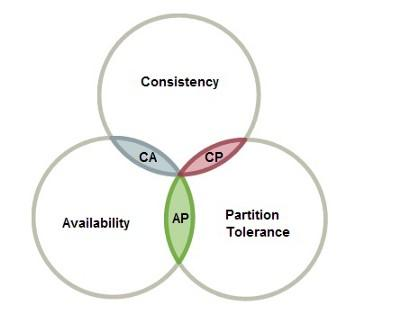
\includegraphics[width=0.3\linewidth]{cap.jpg}
    \caption{Reprezentacja graficzna twierdzenia CAP \cite{cap_rys}}
\end{figure}

Twierdzenie CAP \cite{cap}, odnosi się do trzech podstawowych właściwości, które mogą być gwarantowane w systemach rozproszonych: spójność (Consistency), dostępność (Availability) oraz odporność na rozbicia (Partition Tolerance). Stwierdza ono, że system rozproszony może zapewnić jednocześnie tylko dwie z tych trzech właściwości. Decyzje dotyczące skalowania i zarządzania danymi muszą uwzględniać kompromisy między spójnością, dostępnością i odpornością na rozbicia.

\subsection{Architektura zorientowana na zdarzenia}

Architektura zorientowana na zdarzenia (Event-Driven Architecture, EDA) to podejście, w którym przepływ działania systemu jest sterowany przez zdarzenia - zazwyczaj oznacza to, że działania w systemie są wywoływane w odpowiedzi na konkretne wydarzenia, które mogą być generowane przez różne części aplikacji.

W architekturze mikroserwisowej, gdzie każdy mikroserwis jest odpowiedzialny za określoną funkcjonalność i działa niezależnie, zastosowanie architektury zorientowanej na zdarzenia pozwala na efektywne i elastyczne zarządzanie komunikacją między różnymi serwisami. Oto kilka kluczowych aspektów, jak architektura zorientowana na zdarzenia wspiera tworzenie skalowalnych aplikacji webowych:

\begin{enumerate}
    \item \textbf{Asynchroniczność}: Komunikacja oparta na zdarzeniach jest z natury asynchroniczna. Mikroserwisy mogą emitować zdarzenia bez konieczności oczekiwania na bezpośrednią odpowiedź, co pozwala na bardziej efektywne wykorzystanie zasobów i lepszą skalowalność.

    \item \textbf{Luźne sprzężenie}: Mikroserwisy w architekturze zorientowanej na zdarzenia komunikują się ze sobą głównie poprzez zdarzenia, co minimalizuje bezpośrednie zależności między nimi. To z kolei ułatwia skalowanie, ponieważ zmiany w jednym serwisie rzadziej mają bezpośredni wpływ na inne.

    \item \textbf{Reaktywność i elastyczność}: Systemy zorientowane na zdarzenia mogą szybko reagować na zmiany, co jest kluczowe w dynamicznym środowisku aplikacji webowych. Pozwala to na szybsze dostosowanie się do rosnącego obciążenia czy zmieniających się wymagań biznesowych.

    \item \textbf{Rozproszone przetwarzanie}: Architektura zorientowana na zdarzenia sprzyja rozproszeniu obciążenia przetwarzania. Zamiast obciążać pojedynczy punkt w systemie, zadania mogą być przetwarzane równolegle w różnych mikroserwisach, co zwiększa skalowalność i wydajność.

    \item \textbf{Odporność na awarie}: W przypadku awarii jednego z mikroserwisów, system zorientowany na zdarzenia może lepiej radzić sobie z takimi sytuacjami. Dzięki asynchronicznej komunikacji, pozostałe części systemu mogą kontynuować działanie, co jest kluczowe dla utrzymania ciągłości działania aplikacji.
\end{enumerate}

Podsumowując, architektura zorientowana na zdarzenia, stosowana w ramach architektury mikroserwisowej, znacząco przyczynia się do zwiększenia skalowalności, elastyczności i odporności aplikacji webowych na zmienne warunki i obciążenia.

\subsection{Projektowanie zorientowane na dziedzinę}

Projektowanie zorientowane na dziedzinę (ang. Domain-Driven Design, DDD \cite{ddd}) to podejście do projektowania oprogramowania, które koncentruje się na modelowaniu złożonych systemów biznesowych.

\begin{enumerate}
    \item \textbf{Modelowanie Dziedziny}: DDD skupia się na głębokim zrozumieniu dziedziny biznesowej i jej problemów. W kontekście aplikacji webowych modelowanie dziedziny pomaga w identyfikacji kluczowych funkcji i procesów biznesowych, które aplikacja ma obsługiwać.

    \item \textbf{Język powszechny} (ang. Ubiquitous Language): w DDD to wspólny język, którym posługują się zarówno programiści, jak i eksperci biznesowi. Ułatwia to komunikację i zapewnia, że wszystkie zainteresowane strony mają wspólne rozumienie funkcjonalności aplikacji.

    \item \textbf{Podział na Ograniczone Konteksty }(ang. Bounded Contexts): DDD promuje dzielenie systemu na mniejsze, zarządzane części, znane jako Ograniczone Konteksty. W architekturze mikroserwisowej każdy mikroserwis może reprezentować osobny Kontekst, co pozwala na niezależne zarządzanie, rozwijanie i skalowanie poszczególnych części systemu.

    \item \textbf{Integracja i Komunikacja między Mikroserwisami}: W środowisku mikroserwisowym ważne jest zapewnienie skutecznej komunikacji i integracji między różnymi serwisami. DDD może pomóc w definiowaniu jasnych interfejsów i umów między serwisami, co ułatwia ich integrację i współpracę.

    \item \textbf{Elastyczność i Skalowalność}: Przyjmując podejście DDD w architekturze mikroserwisowej, można osiągnąć większą elastyczność i skalowalność. Mikroserwisy można niezależnie skalować w zależności od potrzeb, co jest szczególnie ważne w przypadku aplikacji webowych, które mogą doświadczać zmiennego obciążenia.

    \item \textbf{Zarządzanie Złożonością}: DDD pomaga w zarządzaniu złożonością poprzez uporządkowanie i systematyzację podejścia do projektowania i implementacji oprogramowania. Pozwala to na efektywniejsze zarządzanie dużymi, skomplikowanymi systemami.

    \item \textbf{Testowanie i Utrzymanie}: DDD ułatwia tworzenie testowalnego i łatwego w utrzymaniu kodu. Jego modularna natura pozwala na izolację i testowanie poszczególnych części systemu niezależnie, co jest kluczowe w skalowalnych aplikacjach webowych.
\end{enumerate}

\subsection{Separacja odpowiedzialności komend i zapytań}

Separacja odpowiedzialności komend i zapytań (ang. Command Query Responsibility Segregation, CQRS \cite{cqrs}) to wzorzec architektoniczny, który rozdziela operacje odczytu (Query) od operacji zapisu (Command) w systemie informatycznym na poziomie architektury. Taka separacja nie wymaga, by oba rodzaje operacji były zaimplementowane w ramach tej samej aplikacji. W przypadku tworzenia skalowalnych aplikacji internetowych CQRS umożliwia efektywniejsze zarządzanie i optymalizację procesów odczytu i zapisu poprzez ich niezależne skalowanie. Wynikiem jest optymalne wykorzystanie zasobów, uproszczenie struktury kodu i zwiększenie ogólnej wydajności systemu. W architekturze opartej na mikroserwisach CQRS dodatkowo sprzyja lepszemu rozdzieleniu obowiązków między poszczególnymi mikroserwisami, co przekłada się na wyższą modułowość i elastyczność systemu.

\begin{figure}[!h]
    \centering 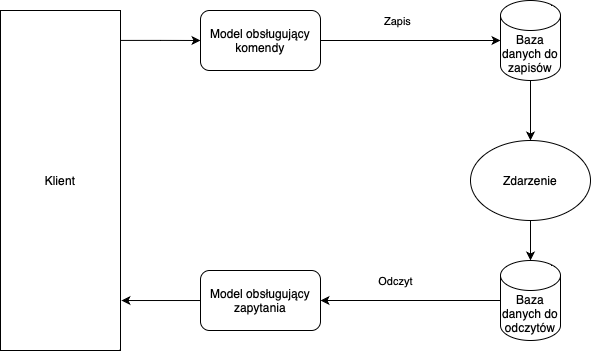
\includegraphics[width=1.0\linewidth]{cqrs.png}
    \caption{Schemat architektoniczny implementacji wzorca CQRS}
\end{figure}

\subsection{Event Sourcing}

Wzorzec Event Sourcing \cite{eventsourcing} jest podejściem w projektowaniu oprogramowania, które polega na przechowywaniu zmian stanu aplikacji jako sekwencji zdarzeń. Każda akcja w systemie generuje zdarzenie, które zamiast modyfikować stan bezpośrednio, jest rejestrowane i służy jako podstawa do odtworzenia bieżącego stanu systemu.

\begin{enumerate}

    \item \textbf{Śledzenie Zmian Stanu}: Event Sourcing umożliwia śledzenie wszystkich zmian stanu systemu poprzez zapisywanie każdego zdarzenia. To podejście zapewnia kompletną historię zmian, co jest szczególnie przydatne w przypadkach wymagających audytu lub debugowania.

    \item \textbf{Odtwarzanie Stanu}: W Event Sourcing stan aplikacji można odtworzyć poprzez przetworzenie sekwencji zdarzeń. Ta zdolność do "odtworzenia przeszłości" jest bardzo cenna w przypadku awarii lub potrzeby analizy historycznych danych, np. podejrzenie stanu systemu na konkretny dzień.

    \item \textbf{Integracja z CQRS}: Event Sourcing często jest stosowany razem z CQRS (Command Query Responsibility Segregation). CQRS oddziela operacje odczytu od zapisu, co w połączeniu z Event Sourcingiem tworzy wydajny i skalowalny model do zarządzania danymi.

    \item \textbf{Złożoność Implementacji}: Jednym z wyzwań stosowania Event Sourcing jest jego złożoność implementacyjna. Wymaga to dokładnego projektowania systemu i może prowadzić do zwiększenia złożoności kodu, szczególnie w przypadku systemów o dużej skali.

    \item \textbf{Zarządzanie Zdarzeniami}: Event Sourcing wymaga skutecznego zarządzania i przetwarzania strumieni zdarzeń, co może być wyzwaniem w dużych systemach. Ważne jest zapewnienie odpowiedniej wydajności i skalowalności mechanizmów przetwarzających zdarzenia, tzw. magazynu zdarzeń i kolejki komunikatów.

    \item \textbf{Odzyskiwanie i Odporność na Awarii}: Wzorzec ten zapewnia naturalną odporność na awarie, ponieważ stan aplikacji może być odtworzony z historii zdarzeń. Jest to szczególnie ważne w środowisku rozproszonym, jakim jest architektura mikroserwisowa.

    \item \textbf{Wersjonowanie Zdarzeń}: W miarę rozwoju systemu, format zdarzeń może się zmieniać. Zarządzanie różnymi wersjami zdarzeń i ich kompatybilnością wsteczną staje się istotnym aspektem projektu.

\end{enumerate}

\begin{figure}[!h]
    \centering 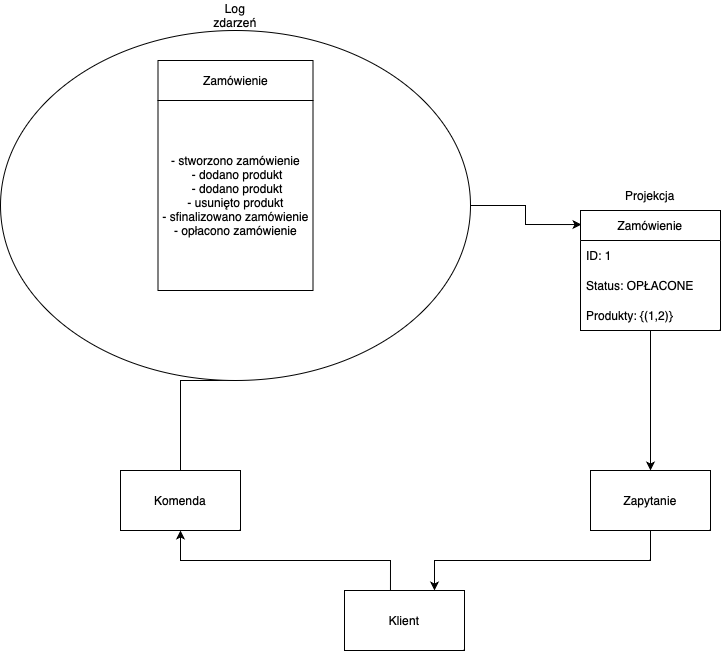
\includegraphics[width=1.0\linewidth]{event_sourcing.png}
    \caption{Schemat architektoniczny implementacji wzorca Event Sourcing}
\end{figure}

\subsection{Wzorzec Saga}

Wzorzec Saga \cite{saga} w architekturze mikroserwisowej jest strategią zarządzania transakcjami rozproszonymi. W systemach opartych na mikroserwisach, gdzie każdy serwis zarządza własną bazą danych, tradycyjne transakcje bazodanowe (jak te stosowane w monolitycznych architekturach) nie są możliwe. Saga oferuje rozwiązanie tego problemu, umożliwiając realizację operacji, które obejmują wiele serwisów, poprzez sekwencję lokalnych transakcji.

\begin{enumerate}

    \item \textbf{Definicja Sag}: Saga to sekwencja operacji, w której każda operacja jest lokalną transakcją w ramach jednego mikroserwisu. Jeśli wszystkie operacje zakończą się pomyślnie, cała Saga jest uznawana za zakończoną sukcesem. Jeśli jednak jedna z operacji zawiedzie, Saga inicjuje serię kompensacyjnych akcji, aby przywrócić system do spójnego stanu.

    \item \textbf{Orkiestracja vs Choreografia}: Istnieją dwa podejścia do implementacji Sag: orkiestracja i choreografia. W orkiestracji centralny koordynator (taki jak serwis orkiestracyjny) zarządza kolejnością i rezultatem operacji. W choreografii każdy mikroserwis zna kolejny krok i samodzielnie publikuje zdarzenia, które są słuchane przez inne serwisy.

    \item \textbf{Kompensacja}: Gdy jedna z operacji w Sadze zawodzi, system musi podjąć akcje kompensacyjne, aby cofnąć zmiany wprowadzone przez poprzednie operacje. Wymaga to starannego projektowania logiki kompensacji dla każdej operacji.

\end{enumerate}
